\documentclass[
    10pt,           % размер шрифта
    aspectratio=43  % соотношение сторон слайдов
]{beamer}

    
%% Tема презентации
\usetheme[]{metropolis}         
\usefonttheme[]{professionalfonts}  % запрещаем beamer'у перезаписывать мат. шрифты

%% Пакеты и их настройки
\usepackage[]{fontspec}         % загрузка шрифтов, работа с кодировкой и пр.
\usepackage[]{polyglossia}      % переносы слов
\usepackage[]{microtype}        % различные исправления типографии
\usepackage[]{unicode-math}     % использование математических символов юникода
\usepackage[]{graphicx}
\usepackage[]{subfig}
\usepackage[]{float}
\usepackage[]{enumitem}
\usepackage[]{tabularx}
\usepackage[]{booktabs}
\usepackage{csquotes} % big quotations
\usepackage[]{caption}
\usepackage[]{subcaption}

\frenchspacing                  %% убираем лишние отступы после точек

%% Перенос слов
\binoppenalty       = 10000 %% Запрет переносов строк в формулах
\relpenalty         = 10000
\pretolerance       = 5000  %% Настройки переноса
\tolerance          = 9000  %% Настройки переноса
\emergencystretch   = 0pt   %% Запрещаем выход за границы
\righthyphenmin     = 2     %% целое число, равное наименьшему количеству букв в слове, которые можно переносить на следующую строку
\lefthyphenmin      = 2
\hyphenpenalty      = 500
\clubpenalty        = 10000 %% Запрет разрывов страниц после первой
\widowpenalty       = 10000 %% и перед предпоследней строкой абзаца

%% Язык
\setmainlanguage[spelling=modern]{russian}
\setotherlanguage{english}

%% Шрифты
\defaultfontfeatures{
    Ligatures  = {TeX, Common},
    Mapping    = tex-text
}

%% Main font
\setmainfont[
    Path            = ./fonts/,
    Extension       = .otf,
    UprightFont     = *-Regular,
    BoldFont        = *-Bold,
    ItalicFont      = *-Italic,
    BoldItalicFont  = *-BoldItalic
]{FreeSerif}
\newfontfamily\cyrillicfont[
    Path            = ./fonts/,
    Extension       = .otf,
    UprightFont     = *-Regular,
    BoldFont        = *-Bold,
    ItalicFont      = *-Italic,
    BoldItalicFont  = *-BoldItalic
]{FreeSerif}

%% Roman font
\setromanfont[
    Path            = ./fonts/,
    Extension       = .otf,
    UprightFont     = *-Regular,
    BoldFont        = *-Bold,
    ItalicFont      = *-Italic,
    BoldItalicFont  = *-BoldItalic
]{FreeSerif}
\newfontfamily\cyrillicfontrm[
    Path            = ./fonts/,
    Extension       = .otf,
    UprightFont     = *-Regular,
    BoldFont        = *-Bold,
    ItalicFont      = *-Italic,
    BoldItalicFont  = *-BoldItalic
]{FreeSerif}

%% Sans font
\setsansfont[
    Path            = ./fonts/,
    Extension       = .otf,
    UprightFont     = *-Regular,
    BoldFont        = *-Bold,
    ItalicFont      = *-Oblique,
    BoldItalicFont  = *-BoldOblique
]{FreeSans}
\newfontfamily\cyrillicfontsf[
    Path            = ./fonts/,
    Extension       = .otf,
    UprightFont     = *-Regular,
    BoldFont        = *-Bold,
    ItalicFont      = *-Oblique,
    BoldItalicFont  = *-BoldOblique
]{FreeSans}

%% Mono font
\setmonofont[
    Path            = ./fonts/,
    Extension       = .otf,
    UprightFont     = *-Regular,
    BoldFont        = *-Bold,
    ItalicFont      = *-Oblique,
    BoldItalicFont  = *-BoldOblique
]{FreeMono}
\newfontfamily\cyrillicfonttt[
    Path            = ./fonts/,
    Extension       = .otf,
    UprightFont     = *-Regular,
    BoldFont        = *-Bold,
    ItalicFont      = *-Oblique,
    BoldItalicFont  = *-BoldOblique
]{FreeMono}

%% Math font
\setmathfont[
    Path        = ./fonts/,
    Extension   = .otf,
    BoldFont    = *Bold
]{XITS-Math}


%% --------------------------------------------------------------
%% Настройки пользователя
%% --------------------------------------------------------------

%% Путь к каталогу с изображениями
\graphicspath{{images/}}
%% Параметры темы
%% http://mirrors.mi.ras.ru/CTAN/macros/latex/contrib/beamer-contrib/themes/metropolis/doc/metropolistheme.pdf
\metroset{
    numbering   = fraction, % нумерация слайдов
    progressbar = frametitle, % информация о прогрессе
    background  = light % светлая тема
}


\title{Разработка и применение алгоритмов определения линейных параметров движущихся объектов методами компьютерного зрения}
%\titlegraphic{\includegraphics[height=1.0cm]{sfedu_logo.png}}
%\subtitle{}

\author{
02.03.02 - Фундаментальная информатика и информационные технологии
\vskip 1em 
Выполнил:\\студент 4 курса И.\,В. Гончаров 
\vskip 1em 
Научный руководитель:\\ к.\,ф.-м.\,н., доцент В.\,В. Махно 
\vskip 1em
}

\date{20 мая 2020 г.}

\institute{Институт ММиКН им. И.И. Воровича, Южный Федеральный Университет}

\begin{document}
    \maketitle
    % !TEX root = ../presentation.tex

\begin{frame}{Общая схема задачи сегментации}
\begin{figure}
\centering
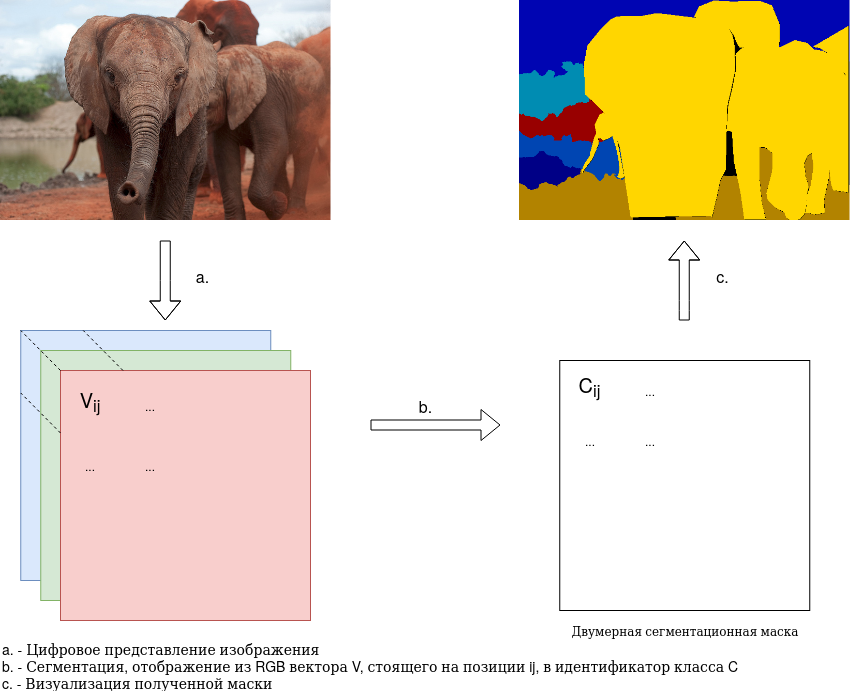
\includegraphics[width=8.51cm, height=6.91cm]{example_segmentation.png}
\end{figure}
%\textbf{$C$}-центр камеры (оптический центр); \textbf{$Cp$}-главная ось камеры
\end{frame}
    % !TEX root = ../presentation.tex

\begin{frame}{Пример задачи сегментации}
\begin{figure}
\centering
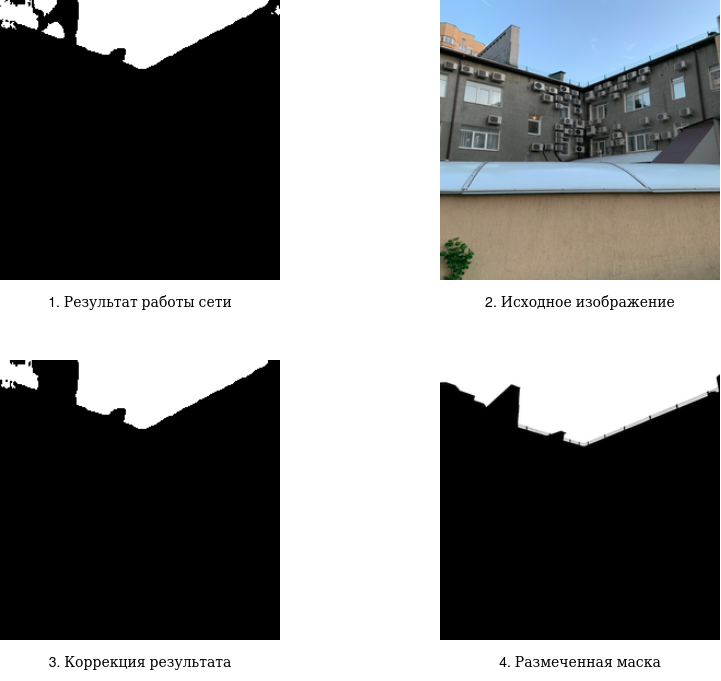
\includegraphics[width=7.21cm, height=6.81cm]{sky_segmentation.png}
\end{figure}
%\textbf{$C$}-центр камеры (оптический центр); \textbf{$Cp$}-главная ось камеры
\end{frame}
    % !TEX root = ../presentation.tex

\begin{frame}{Общий вид FCN}
\begin{figure}
\centering
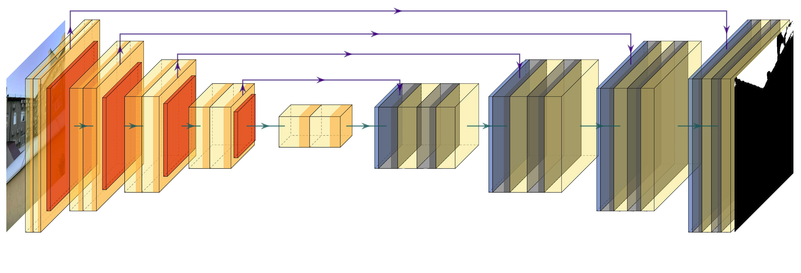
\includegraphics[width=9.01cm, height=3.73cm]{net_arch.png}
\end{figure}
    Энкодер и декодер части сети.
    Такой подход позволяет выделить признаки, а затем генерализировать их для классификации.
%\textbf{$C$}-центр камеры (оптический центр); \textbf{$Cp$}-главная ось камеры
\end{frame}
    % !TEX root = ../presentation.tex

\begin{frame}{Метрика}
\begin{figure}
\centering
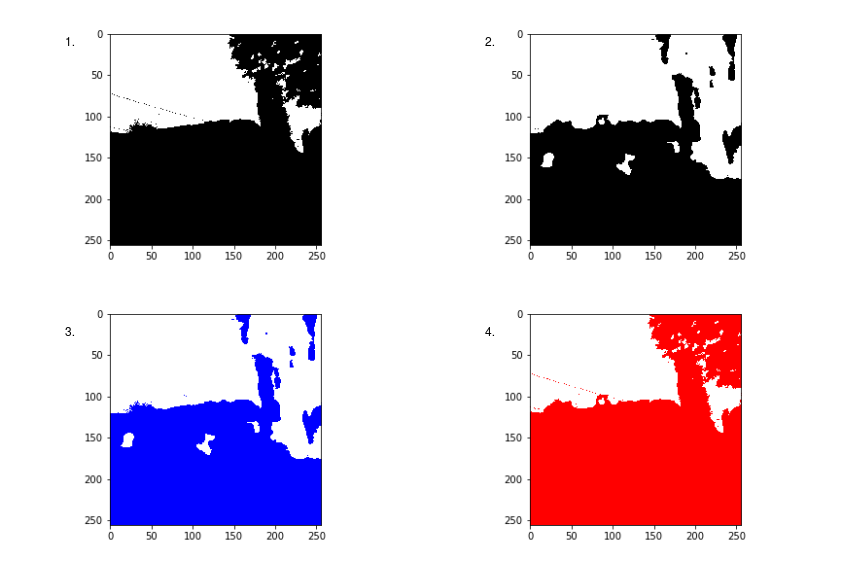
\includegraphics[width=8.41cm, height=6.91cm]{iou_vis.png}
\end{figure}
%\textbf{$C$}-центр камеры (оптический центр); \textbf{$Cp$}-главная ось камеры
\end{frame}
    % !TEX root = ../presentation.tex

\begin{frame}{Примеры изображений SkyFinder}
\begin{figure}
\centering
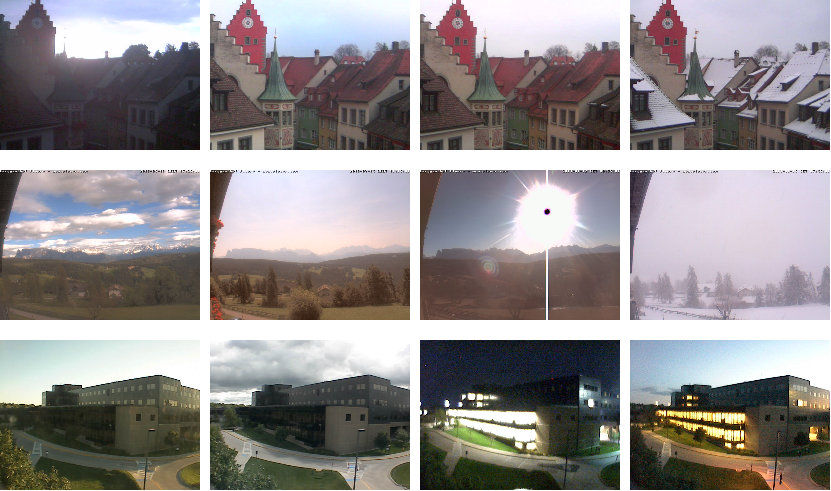
\includegraphics[width=8.31cm, height=4.91cm]{skyfinder.png}
\end{figure}
%\textbf{$C$}-центр камеры (оптический центр); \textbf{$Cp$}-главная ось камеры
\end{frame}
    % !TEX root = ../presentation.tex

\begin{frame}{Нормализация по пакету}
\begin{figure}
\centering
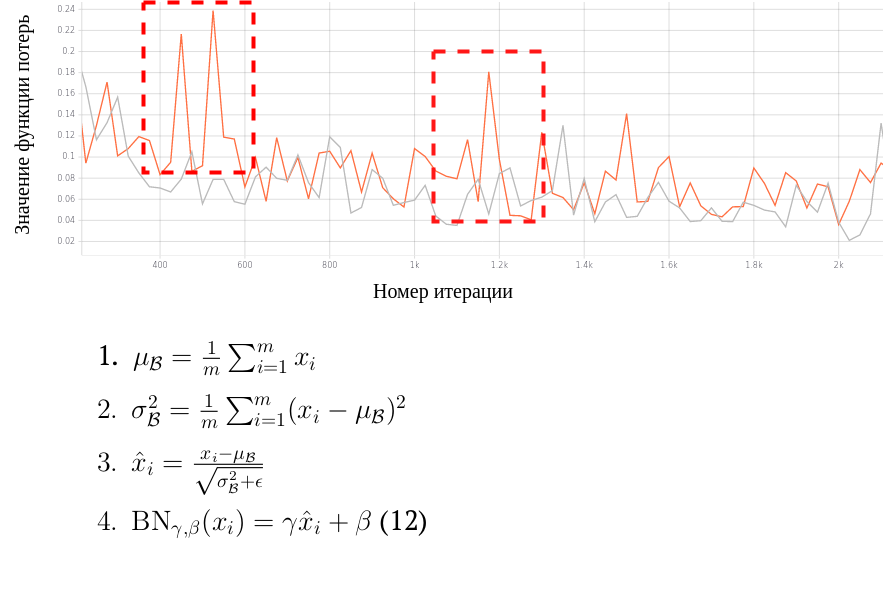
\includegraphics[width=9.11cm, height=6.50cm]{batch_normalization_pres.png}
\end{figure}
    Оранжевым цветом отражен процесс обучеения без нормализации, серым - с нормализацией.
%\textbf{$C$}-центр камеры (оптический центр); \textbf{$Cp$}-главная ось камеры
\end{frame}
    % !TEX root = ../presentation.tex

\begin{frame}{Softmax}
\begin{figure}
\centering
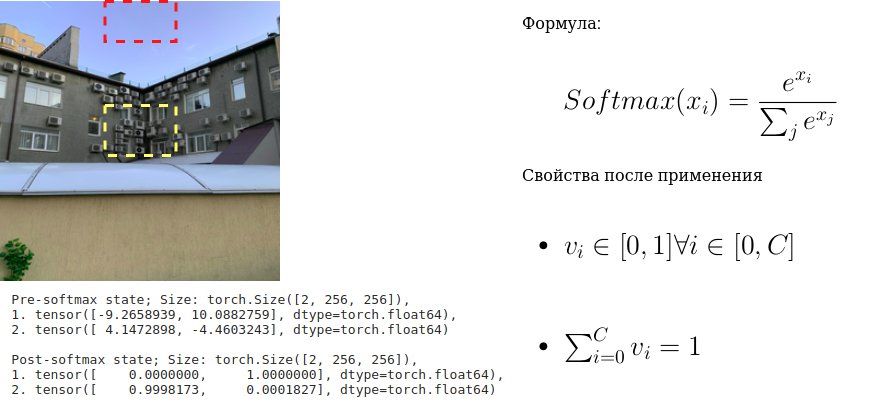
\includegraphics[width=9.79cm, height=5.08cm]{softmax_debug_info_pres.png}
\end{figure}
%\textbf{$C$}-центр камеры (оптический центр); \textbf{$Cp$}-главная ось камеры
\end{frame}
    % !TEX root = ../presentation.tex

\begin{frame}{Выходы декодер-части}
\begin{figure}
\centering
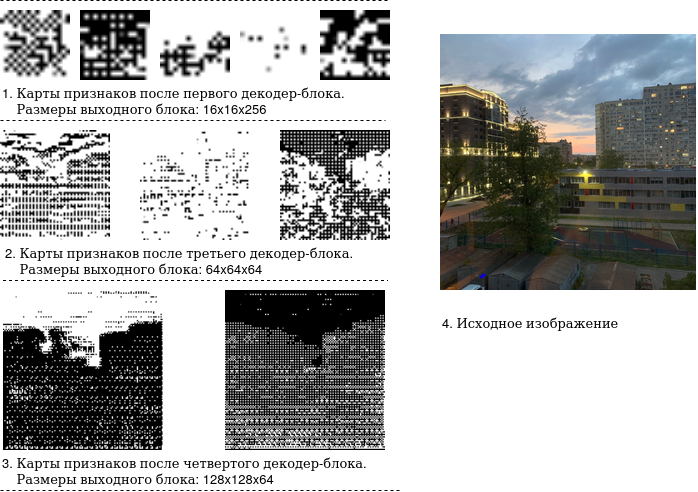
\includegraphics[width=6.98cm, height=4.92cm]{decoder_outputs.png}
\end{figure}
%\textbf{$C$}-центр камеры (оптический центр); \textbf{$Cp$}-главная ось камеры
\end{frame}
    % !TEX root = ../presentation.tex

\begin{frame}{Оптимизация функции потерь}
\begin{figure}
\centering
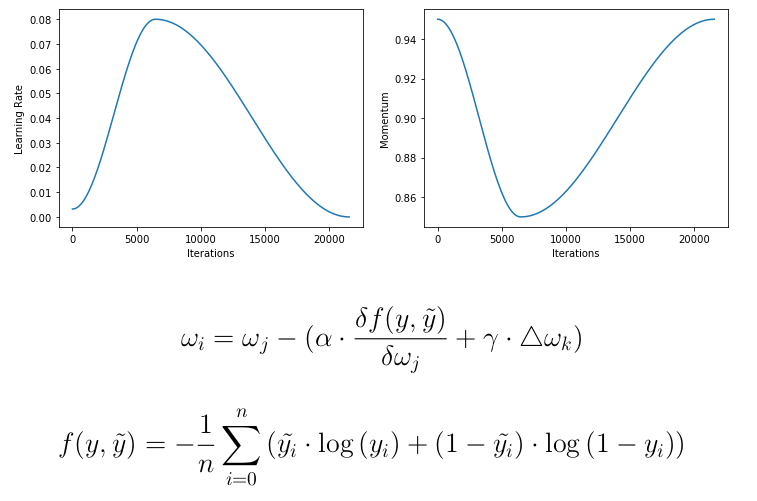
\includegraphics[width=7.57cm, height=5.01cm]{ocp.png}
\end{figure}
%\textbf{$C$}-центр камеры (оптический центр); \textbf{$Cp$}-главная ось камеры
\end{frame}
    % !TEX root = ../presentation.tex

\begin{frame}{Сравнение процессов обучения}
\begin{figure}
\centering
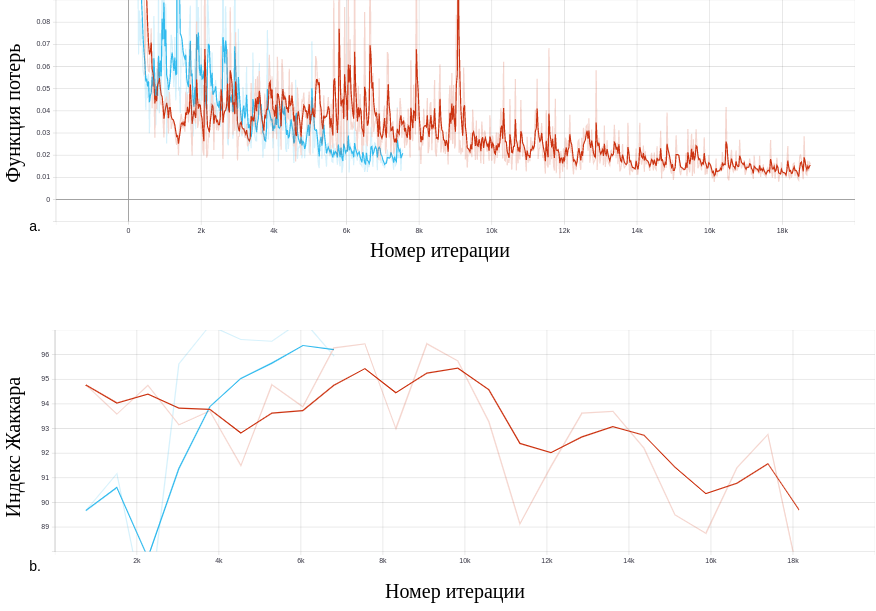
\includegraphics[width=8.41cm, height=7.36cm]{ocp_against_const.png}
\end{figure}
%\textbf{$C$}-центр камеры (оптический центр); \textbf{$Cp$}-главная ось камеры
\end{frame}
    \begin{frame}{Пример работы на ректифицированном изображении}
\begin{figure}
    \centering
    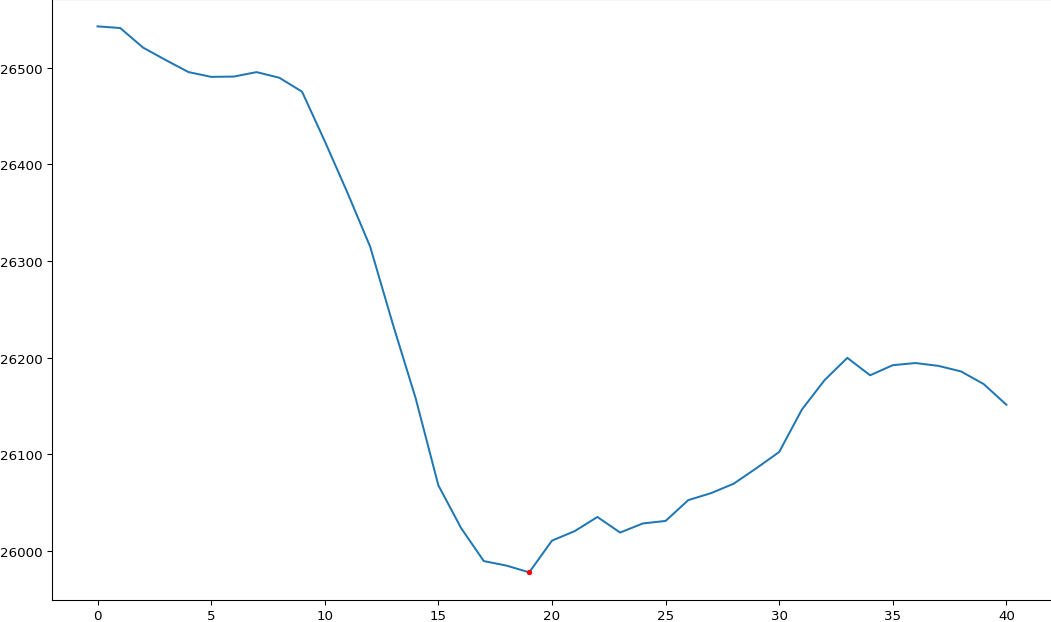
\includegraphics[width=\textwidth]{undistorted-sample.png}
\end{figure}
\end{frame}
    % !TEX root = ../presentation.tex

\begin{frame}{Сравнение результатов сети}
\begin{figure}
\centering
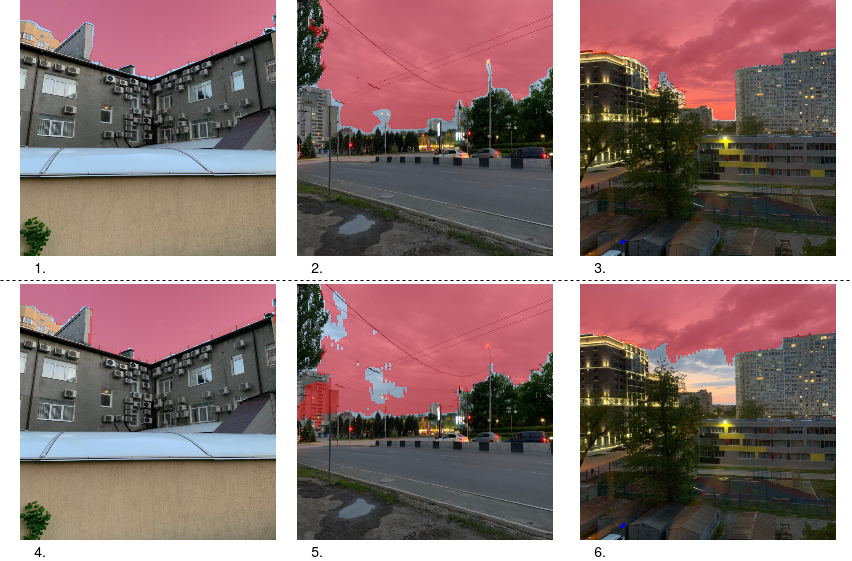
\includegraphics[width=8.52cm, height=5.61cm]{data_count_compare.png}
\end{figure}
%\textbf{$C$}-центр камеры (оптический центр); \textbf{$Cp$}-главная ось камеры
\end{frame}
    % !TEX root = ../presentation.tex

\begin{frame}{Результаты работы}
\begin{block}{}
    В рамках данной работы сделано:
\begin{itemize}
    \item Спроектирована и реализована архитектура сети для решения задачи сегментации
    \item Реализована возможность обучения с использованием техники one cycle policy
    \item Реализована возможность синтетической разметки датасета
    \item Реализована для экспериментов обучения загрузчик данных из нескольких источников с выбором количественного отношения
\end{itemize}
    Ссылка на репозиторий проекта: https://github.com/DmitIW/BachelorDiploma
\end{block}
%\textbf{$C$}-центр камеры (оптический центр); \textbf{$Cp$}-главная ось камеры
\end{frame}
    \begin{frame}{Пример получаемых результатов}
\begin{figure}
    \centering
    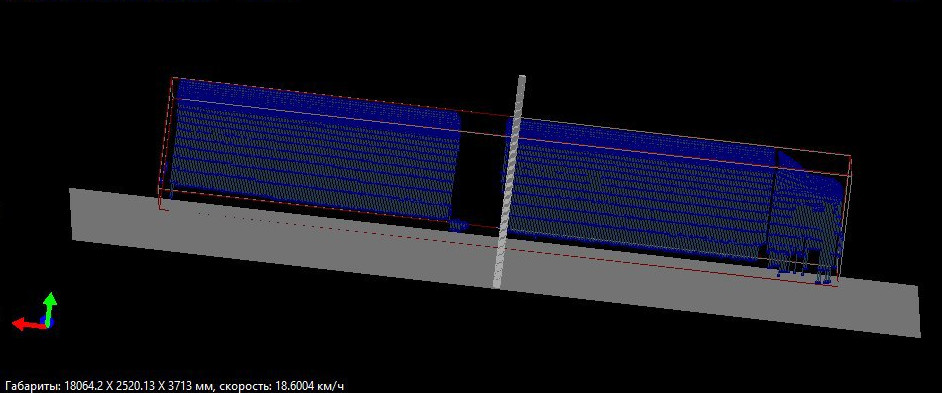
\includegraphics[width=\textwidth]{vhdc-cloud-sample-2.JPG}
\end{figure}
\end{frame}
\end{document}